%%%%%%%%%%%%%%%%%%%%%%% CHAPTER - 3 %%%%%%%%%%%%%%%%%%%%\\
\chapter{System Analysis}
\label{C3} %%%%%%%%%%%%%%%%%%%%%%%%%%%%
\graphicspath{{Figures/Chapter-3figs/PDF/}{Figures/Chapter-3figs/}}
% \noindent\rule{\linewidth}{2pt}
%%%%%%%%%%%%%%%%%%%%%%%%%%%%%%%%%%%%%%%%%%%%%%%%%%%%%%%%%%%%%%%%%%%%%%%%%%%%%%%%%%
The system analysis phase involves examining the functional and non-functional requirements, design constraints, feasibility aspects, and hardware/software needs of the proposed system. This chapter provides a detailed analysis of the AI-powered Cricket Batting Analysis System, a real-time image classification and feedback system that utilizes deep learning and computer vision techniques to improve cricket training efficiency, accuracy, and accessibility through a client–server architecture.
	%%%%%%%%%%%%%%%%%%%%%%%%%%%%%%%%%%%%%%%%%%%%%%%%%%%%%%%%%%%%%%%%%%%%%%%%%%%%%%%%%%
\section{Functional Requirements} \label{S3.1}
The proposed AI-Powered Cricket Batting Analysis System is expected to meet the following functional requirements:

\noindent\textbf{FR 1:} Capture Player Image\\
\textit{Description:} The system should capture a clear image of the player’s batting stance using the Android mobile camera integrated through CameraX. The application must provide a live preview and allow the user to focus before capturing the image.\\
\textit{Input:} Live camera feed from the mobile device.\\
\textit{Output:} High-quality captured batting image stored temporarily in device storage. \\

\noindent\textbf{FR 2:} Preprocess Captured Image\\
\textit{Description:} The system should preprocess the captured image to make it suitable for deep learning model inference. This includes resizing the image to the required dimensions (e.g., 224×224), correcting orientation, and normalizing pixel values.\\
\textit{Input:} Raw captured image file.\\
\textit{Output:} Preprocessed image ready for transmission and model prediction.\\

\noindent\textbf{FR 3:} Upload Image to Backend Server\\
\textit{Description:} The Android application should securely transmit the preprocessed image to the backend server using a multipart HTTP POST request through Retrofit. The system must support dynamic server IP configuration to ensure flexibility.\\
\textit{Input:} Preprocessed image file.\\
\textit{Output:} Successful image upload to the server endpoint.\\

\noindent\textbf{FR 4:} Perform Shot Classification\\
\textit{Description:} The backend server should load the trained deep learning model and perform classification on the received image. The system must accurately identify the batting shot category or label it as unknown if it does not match trained classes.\\
\textit{Input:} Uploaded batting image.\\
\textit{Output:} Predicted shot category with confidence score.\\

\noindent\textbf{FR 5:} Generate Annotated Output\\
\textit{Description:} After prediction, the server should generate a processed or annotated image (if applicable) and convert it into Base64 format for easy transmission back to the client application.\\
\textit{Input:} Model prediction result.\\
\textit{Output:} Base64-encoded processed image along with classification label in JSON format.\\

\noindent\textbf{FR 6:} Display Visual Feedback\\
\textit{Description:} The Android application should receive the server response and display the predicted shot category clearly n the screen along with the processed image overlay. The UI should be responsive and user-friendly.\\
\textit{Input:} JSON response from server.\\
\textit{Output:} Visual representation of prediction result.\\

\noindent\textbf{FR 7:} Provide Audio Feedback\\
\textit{Description:} The system should use Text-to-Speech functionality to announce the predicted shot category, ensuring accessibility and interactive feedback for users during practice sessions.\\
\textit{Input:} Predicted shot label.\\
\textit{Output:} Clear voice output informing the user of the classification result.\\

\noindent\textbf{FR 8:} User Authentication (Login and Logout)\\
\textit{Description:} The system should allow users to securely log in using their email and password to access the AI Cricket Coach application and provide a logout option to end the session safely.\\
\textit{Input:} User email address and password.\\
\textit{Output:} Successful login grants access to the application, while logout securely ends the session and returns to the login screen.\\


%%%%%%%%%%%%%%%%%%%%%%%%%%%%%%%%%%%%%%%%%%%%%%%%%%%%%%%%%%%%%%%%%%%%%%%%%%%%%%%%%%%%%%%%%%%%%%%%%%%%%%%%%%%%%%%%%%%%%%%%%%%%%%%%%
\section{Non-functional Requirements}	\label{S3.2}
The proposed AI Cricket Coach system must also satisfy the following non-functional
requirements to ensure reliability and user satisfaction.\\
\noindent\textbf{NFR 1: Availability:} The system should be available for the user 24×7 without failure.\\
\noindent\textbf{NFR 2: Reliability:} The system should be reliable with failure free operations. The reliability value ranges from 0 to 1.\\
\noindent\textbf{NFR 3: Maintainability:} The system should be maintainable without changing the base structure.\\
\noindent\textbf{NFR 4: Security:} The system should not be vulnerable to the attackers. The data gathered and stored by the system should be secure.

%%%%%%%%%%%%%%%%%%%%%%%%%%%%%%%%%%%%%%%%%%%%%%%%%%%%%%%%%%%%%%%%%%%%%%%%%%%%%%%%%%%%%%%%%%%%%%%%%%%%%%%%%%%%%%%%%%%%%%%%%%%%%%%%%
%%%%%%%%%%%%%%%%%%%%%%%%%%%%%%%%%%%%%%%%%%%%%%%%%%%%%%%%%%%%%%%%%%%%%%%%%%%%%%%%%%%%%%%%%%%%%%%%%%%%%%%%%%%%%%%%%%%%%%%%%%%%%%%%%
\section{Feasibility Analysis}  \label{S3.3}
Feasibility analysis evaluates whether the proposed AI-Powered Cricket Batting Analysis System is practical, implementable, and beneficial within given constraints. It examines the technical capability, operational practicality, and economic viability of developing and deploying the system. This ensures that the project can be successfully implemented using available resources and technologies.

\subsection{Technical Feasibility}  
Technical feasibility assesses whether the required technology, tools, and technical expertise are available to develop the system.
The proposed system is technically feasible as it utilizes widely available and proven technologies such as Python, Flask for model training, and Android Studio for mobile application development. The deep learning model was successfully trained using Google Colab, which provides sufficient computational power for model development. The backend server can be executed in VS Code using standard hardware with moderate specifications.
The Android application uses CameraX for image capture and Retrofit for server communication, both of which are well-supported and stable libraries. Since the system follows a client–server architecture, heavy computations are performed on the server, reducing the processing burden on the mobile device. Therefore, from a technological perspective, the system is practical and achievable.

\subsection{Operational Feasibility}
Operational feasibility determines whether the system will function effectively in real-world conditions and whether users can operate it easily.
The system is designed to be user-friendly and accessible. Players simply need to open the Android application, capture an image, and receive instant feedback. No specialized technical knowledge is required to operate the system. The interface is simple, interactive, and provides both visual and audio feedback to enhance usability.
The solution can be used in cricket academies, schools, or personal practice sessions. Since the system works with standard smartphones and does not require expensive motion-tracking hardware, it is practical for everyday training use. Thus, the system is operationally feasible and suitable for real-world deployment.

\subsection{Economic Feasibility}
Economic feasibility evaluates whether the project is cost-effective and financially viable.
The proposed system is economically feasible because it uses open-source tools and platforms such as Python, Flask, and Android Studio. Model training was performed using Google Colab, which offers free computational resources. The system does not require expensive sensors, motion-capture devices, or specialized hardware.
Only a standard smartphone and a basic computer for server deployment are needed. This significantly reduces overall implementation cost compared to traditional motion-tracking or advanced sports analytics systems. Therefore, the project provides a cost-effective solution for AI-based cricket training.
%%%%%%%%%%%%%%%%%%%%%%%%%%%%%%%%%%%%%%%%%%%%%%%%%%%%%%%%%%%%%%%%%%%%%%%%%%%%%%%%%%%%%%%%%%%%%%%%%%%%%%%%%%%%%%%%%%%%%%%%%%%%%%%%%
%%%%%%%%%%%%%%%%%%%%%%%%%%%%%%%%%%%%%%%%%%%%%%%%%%%%%%%%%%%%%%%%%%%%%%%%%%%%%%%%%%%%%%%%%%%%%%%%%%%%%%%%%%%%%%%%%%%%%%%%%%%%%%%%%
\section{Hardware Requirements}  \label{S3.4}
To ensure optimal performance and seamless functionality of the AI-Powered Cricket Batting Analysis System, certain hardware components are essential. The following hardware resources were utilized for system development, training, deployment, and testing:

\begin{itemize}	
	\item Laptop or Desktop Computer (minimum 8GB RAM, Intel i5 or equivalent processor) for model training, server execution, and development in VS Code
	\item Android Smartphone (with minimum Android 8.0 and functional rear camera) for running the mobile application
	\item High-Resolution Smartphone Camera (minimum 8MP recommended) for capturing clear batting images
	\item Stable Internet Connection (Wi-Fi or Mobile Data) for client–server communication and real-time image upload
	\item Cloud-Based Platform (Google Colab) for deep learning model training using GPU resources
	\item External Storage (optional) for dataset storage containing 8000+ images
	\item Audio Output Device (mobile speaker or headset) for Text-to-Speech feedback
\end{itemize}

These hardware components ensure smooth image capture, efficient server communication, accurate model inference, and proper feedback delivery during cricket training sessions.
%%%%%%%%%%%%%%%%%%%%%%%%%%%%%%%%%%%%%%%%%%%%%%%%%%%%%%%%%%%%%%%%%%%%%%%%%%%%%%%%%%%%%%%%%%%%%%%%%%%%%%%%%%%%%%%%%%%%%%%%%%%%%%%%%
\section{Software Requirements}  \label{S3.5}
The primary software tools and technologies used in the development of the AI-Powered Cricket Batting Analysis System include:

\begin{itemize}
	\item Operating System: Windows / macOS / Linux
	\item Programming Languages: Python (Backend and Model), Java (Android Application)
	\item Frameworks: Flask (Backend Server), Android SDK
	\item AI Libraries: YOLOv8, XGBoost
	\item Deep Learning Platform: Google Colab (for model training with GPU support)
	\item Networking Library: Retrofit (for client–server communication)
	\item Database/Storage: Local storage for dataset (optional cloud storage for backup)
	\item Development Environment: Visual Studio Code (Server), Android Studio (Mobile App), Google Colab (Model Training)
\end{itemize}

These software components collectively support dataset preparation, model training, backend deployment, mobile application development, and real-time shot classification functionality.
%%%%%%%%%%%%%%%%%%%%%%%%%%%%%%%%%%%%%%%%%%%%%%%%%%%%%%%%%%%%%%%%%%%%%%%%%%%%%%%%%%%%%%%%%%%%%%%%%%%%%%%%%%%%%%%%%%%%%%%%%%%%%%%%%
\section{Life Cycle Used}  \label{S3.6}
In this project, we chose the Agile model. It is an iterative and incremental development 
approach. We develop our project as different modules, which are completed in multiple 
sprints. The Agile model shown in Figure 3.1 is flexible and makes it easier to incorporate new features and improvements during the development phase.

\begin{figure}[h]
	\centering
	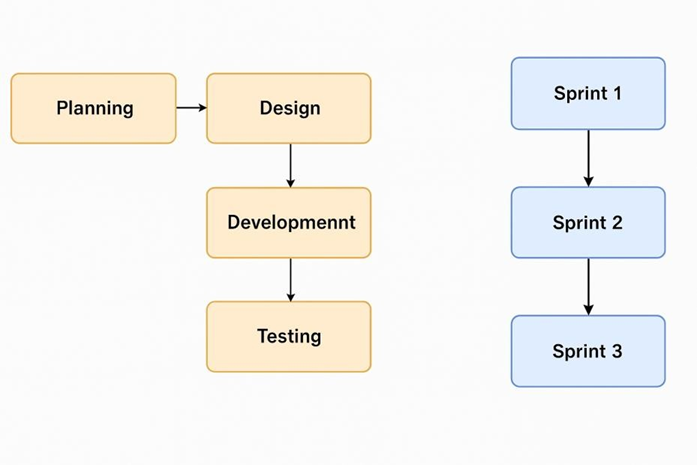
\includegraphics[width=0.5\linewidth]{Figures/Chapter-3figs/agile_model}
	\caption{Agile Model}
	\label{fig:agile}
\end{figure}

Analogous to the role of the software-development lifecycle (SDLC), the machine learning 
model-development lifecycle (MDLC) guides the activities of ML model development from 
inception through retirement. The key phases of the MDLC including data ingestion, 
exploratory data analysis, model creation, and model operation are illustrated in Figure 3.2.

\begin{figure}[h]
	\centering
	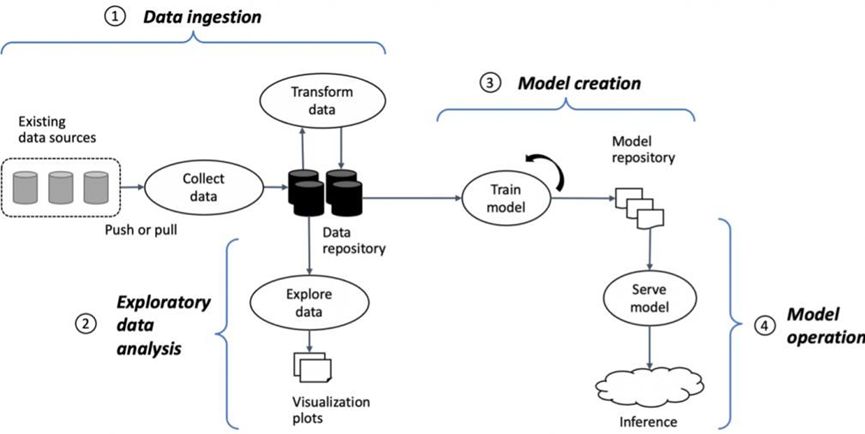
\includegraphics[width=0.7\linewidth]{Figures/Chapter-3figs/mdlc_model}
	\caption{MDLC Model}
	\label{fig:screenshot003}
\end{figure}

\section{Software Cost Estimation} \label{S3.7}
\begin{table}[H]
	\centering
	\caption{COCOMO model coefficients}
	\label{tab:cocomo}
	
	\begin{tabular}{|l|c|c|c|c|}
		\hline
		\rowcolor[gray]{0.85}
		\textbf{Software Category} & \textbf{a} & \textbf{b} & \textbf{c} & \textbf{d} \\
		\hline
		Organic & 2.4 & 1.05 & 2.5 & 0.38 \\
		\hline
		Semi-detached & 3.0 & 1.12 & 2.5 & 0.35 \\
		\hline
		Embedded & 3.6 & 1.20 & 2.5 & 0.32 \\
		\hline
	\end{tabular}
	
\end{table}
\textbf{Software Project Category:} Organic\\  
\textbf{Estimated Lines of Code (LOC):} 3500 LOC   = 3.5 KLOC\\
\textbf{Effort applied} = a*(KLOC)b [Person-Months] = 2.4(3.5)1.05 = 8.94 PM (Person-Months)\\
\textbf{Development Time} = c*(Effort)d = 2.5(8.94)0.38 = 5.74 months / 175 days\\
\textbf{No: of Persons} = Effort / Development Time = 8.94 / 5.74 = 1.55 = 2 person\\

\section{Total Product Cost Estimation}  \label{S3.9}
The total product cost is the sum of both hardware and software costs involved in developing 
the AI Cricket Coach system. As this project uses certain premium tools and cloud-based 
services like Google Colab Pro for AI model training and testing.\\The estimated cost 
for developing this project is:\\
\textbf{Total cost} = Hardware cost + Software cost = 0 + 6000 =6000 INR

\section{Project Schedule using Gantt chart}  \label{S3.10}
\begin{figure}[H]
	\centering
	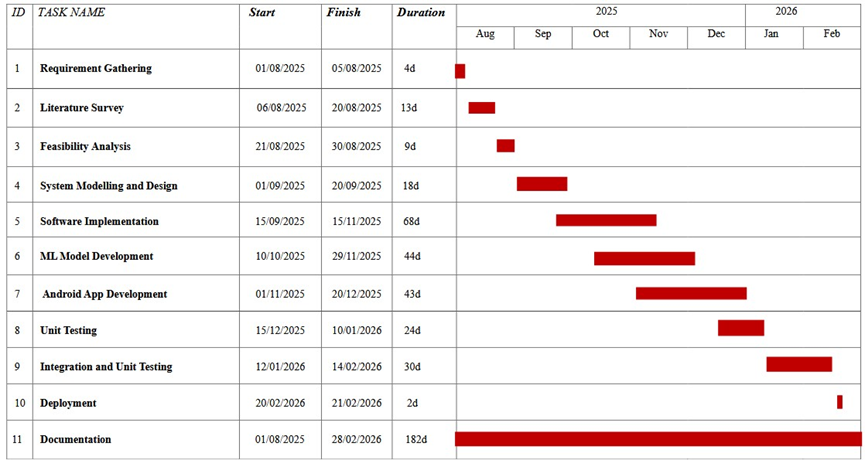
\includegraphics[width=1.05\linewidth]{Figures/Chapter-3figs/gantt_chart}
	\caption{Project Schedule using Gantt chart}
	\label{fig:gantt_chart}
\end{figure}
The Gantt chart shows the project scheduling. Gantt chart shows the start and finish date of the 
project. Our project phases will be completed as per the prescribed time schedule in the above 
Gantt chart shown in Figure 3.3. The starting date was 01/08/2025 and the project is expected 
to complete on 28/02/2026.